\documentclass[runningheads]{llncs}

\usepackage{graphicx}
\usepackage{amsmath,amssymb}
\usepackage{booktabs}
\usepackage{multirow}
\usepackage{algorithm}
\usepackage{algorithmic}
\usepackage[hidelinks]{hyperref}
\usepackage{xcolor}
\usepackage[UTF8,fontset=none]{ctex}
\setCJKmainfont{Songti SC}
\setCJKsansfont{STHeiti}
\setCJKmonofont{Songti SC}

\newcommand{\ie}{\textit{i.e.}}
\newcommand{\eg}{\textit{e.g.}}

\begin{document}

\title{让资源行动可观测：基于AEIC结构化报告的\\多智能体大语言模型审议机制设计}

\titlerunning{博弈驱动的可观测语义共识机制}

\author{Tiancheng Ma\inst{1}}
\authorrunning{T. Ma}

\institute{School of Computer Science\\
\email{author@university.edu}}

\maketitle

\begin{abstract}
多智能体语言模型系统通常优化最终聚合结果，却很少观测产生该结果的行为。当完整独立报告比短答案或模仿具有更高成本时，系统无法区分真实审议与低成本一致。本文提出\emph{AEIC-MD}：以假设--证据--推理--结论（AEIC）报告作为机制设计者与LLM Agent之间可观测接口的审议框架。求解前，每个Agent观察公开信用--成本规则，并从低资源报告、完整AEIC推理、追加验证和同伴模仿中选择行动；行动控制真实生成过程，并在结算前写入日志，从而可以直接检验追随者响应。

在StrategyQA、MMLU-Hard和TruthfulQA的450道配对测试题上，静态AEIC规则将高资源行动率从0.46\%提高到56.93\%，多数投票准确率从68.00\%提高到82.22\%（$+14.22$个百分点；Holm校正McNemar $p=1.23\times10^{-11}$）。仅结果奖励只将高资源行动率提高到3.08\%，且未改善准确率（67.33\%，$p=0.780$）。奖励和成本扫描呈现预期单调响应；受控信息环境、额外Seed、信号与历史消融以及3--5 Agent面板限定了稳健性。留出GLM后端未复现行动或准确率增益（69.33\%对70.67\%，$p=0.791$），表明合同必须针对后端校准。八组预注册实验共包含5,850条经核验的问题级记录。结果支持有边界的结论：针对可验证报告结构的公开规则能够改变追随者资源行动并改善集体决策，但合同语义不会自动跨模型家族迁移。
\keywords{多智能体大语言模型 \and 机制设计 \and 结构化推理 \and 群体审议 \and 追随者响应}
\end{abstract}

\section{引言}\label{sec:intro}
LLM Agent能够辩论、批评、投票并综合彼此输出，但聚合结果的价值取决于产生它的行为。短答案、独立推理报告、追加验证和模仿同伴具有不同成本与信息价值。多数评测只观察最终答案，使系统无法区分真实审议与廉价一致。

这首先是机制设计问题，其次才是聚合问题。设计者必须在Agent行动前宣布何种行为获得信用，Agent再决定预期信用是否值得资源投入。对既有回答做回溯加权不能建立追随者响应，因为生成策略未观察该规则；改变拓扑也只能控制信息流向，不能决定Agent是否生产可独立检查的信息。

本文提出\textbf{博弈驱动的可观测语义共识机制}，并以Assumption、Evidence、Inference和Conclusion四个可解析字段构成的AEIC报告作为观测接口。求解前，追随者观察包含信用规则、行动成本、信息策略和验证预算的公开合同，并从Low、AEIC、Verify和Imitate中选择。行动选择真实生成路径；报告、资源、信用、成本和信誉更新均被记录。这把“先承诺、后响应”的Stackelberg直觉转化为可证伪实验。AEIC负责使过程可解析和可结算，机制处理则是行动前合同及其与真实资源路径的绑定。

确认性实验在三个任务域的450道留出题上配对比较三种规则。Static AEIC将高资源行动率从0.46\%提高到56.93\%，联合执行配置下的准确率从68.00\%提高到82.22\%；Outcome Only仅提高到3.08\%，准确率无显著变化。因此现有结果支持局部可读过程规则改变行动策略，但由于条件同时改变执行提示、Token和后端路由，质量增益不能单独归因于AEIC格式或信用文本。

本文还用奖励--成本扫描、四类信息环境、信号与历史消融、额外Seed、不同面板规模和留出GLM后端检验解释。GLM未响应同一合同，这一负结果排除普适性强主张，并将后端合同校准确定为开放问题。

本文贡献为：\begin{enumerate}
\item 可执行Leader--Follower协议：规则先于行动，行动控制真实资源路径；
\item 配对证据表明基于AEIC观测接口的过程合同相对仅结果奖励能够改变资源行动，并在联合执行配置下伴随集体准确率改善；
\item 完整冻结的八组评测，覆盖剂量响应、信息控制、消融、稳健性和明确的不迁移边界。
\end{enumerate}

\section{相关工作}\label{sec:related}

\subsection{多样化采样、投票与多智能体审议}
提高测试时计算量的早期路线主要依赖多次采样和结果聚合。Self-consistency对同一问题生成多条推理路径并以答案频率聚合~\cite{wang2023selfconsistency}；选举式集体决策进一步用不同投票规则维护候选多样性~\cite{zhao2024electoral}。这类方法能够利用独立采样降低单次生成波动，但默认各样本已经完成了足够的信息生产，通常不区分短答、独立证据和追加验证的成本。

多智能体辩论把聚合前的独立样本扩展为跨轮交互。Du等让多个模型实例提出答案、交换论证并在多轮后形成结果~\cite{du2024improving}；FORD研究模型能力不平衡时的跨模型一致性和强模型支配~\cite{xiong2023interconsistency}；ChatEval、AgentVerse和角色化系统把讨论者、批评者或评估者组织成任务流程~\cite{chan2023chateval,chen2023agentverse}。后续工作从人格、反思和辩论模式研究协作效率~\cite{zhang2024collaboration}，也比较辩论、投票和动态加权共识~\cite{choi2025debate,li2025dynamic}。这些工作主要回答“Agent怎样交换和聚合既有输出”，本文则将研究对象前移为“规则如何改变输出产生前的行动与资源路径”。

\subsection{从众、异议损失与通信风险}
交互并不必然改善决策。已有研究发现同质模型容易出现谄媚、从众和过早一致，正确少数意见可能在多轮讨论中消失~\cite{pitre2025consensagent,swamy2025peacemaker}；共识与多样性之间存在任务相关权衡~\cite{wu2025disagreement}。对抗性协作研究进一步表明，具有较强说服力的错误Agent能够通过辩论影响其他成员~\cite{amayuelas2024multiagent}。因此，通信轮数、拓扑或多数票本身不能证明有效审议：系统还需要记录谁看到了什么、何时改变立场、改变是否伴随新证据，以及各候选是否接受了相同覆盖。

本文不把通信拓扑作为主因果变量。确认性实验固定同步面板与信息流，只改变行动前公开规则；受控信息实验再分别提供新增证据、无证据多数立场、复制压力和反向证据。该设计与从众研究互补：现有工作刻画错误如何传播，本文检验可观察过程合同是否能够改变传播之前的信息生产行为。

\subsection{结构化推理、验证与可观察报告}
Chain-of-Thought显式化中间步骤，Tree-of-Thoughts把求解组织为搜索，ReAct把推理与外部行动交替执行~\cite{wei2022chain,yao2024tree,yao2023react}。这些方法说明中间结构有助于分解复杂任务和连接工具，但结构化文本不自动等于事实正确，也不保证报告来自独立验证。自由文本评审还存在字段缺失、结论难以规范化和证据来源无法定位的问题。

AEIC与上述方法的关系是“审计接口”而非新的隐式思维链。它只保存假设、证据、推断和结论四类可公开短报告，并把字段完整、结论合法、证据增量、核验证据、有用纠正和无支持翻转转换为可结算信号。本文额外设置自由文本、通用“分析--答案”结构和AEIC的等预算比较，以避免把一般结构化输出的收益错误归因于AEIC字段命名。

\subsection{LLM中的机制设计与委托代理视角}
机制设计研究关注设计者先承诺规则、参与者随后根据规则行动。已有工作在生成内容拍卖中研究由LLM表示偏好的机制与单调性条件~\cite{duetting2023mechanism}，在文本生成中使用统计合同激励可测质量~\cite{saig2024incentivizing}，并从委托--代理和信息不对称角度讨论多Agent系统~\cite{rauba2025principal,kaltenpoth2025agency}。Stackelberg激励也广泛用于联邦学习、众包和资源分配~\cite{fu2024stackelberg,guo2023incentive,wang2024incentive}。

与生成后评分不同，本文要求合同在求解前进入Follower可见上下文，并使声明行动选择不同Prompt、Token上限、调用次数和验证路径。经验对象是黑盒模型在固定合同下产生的行动分布，而不是预设其具有稳定的人类效用。我们使用Stackelberg时序组织实验，但不声称求得闭式均衡、一般激励相容或全局最优合同。

\subsection{本文定位}
现有多智能体研究已经较充分地覆盖角色分工、通信拓扑、辩论轮次、投票规则和裁判模型；结构化推理研究解决中间过程表达；机制设计研究提供先承诺后响应的分析框架。三者之间仍缺少一个可执行连接：公开规则必须在生成前可见，行动必须真实控制资源路径，自然语言报告必须成为可解析结算对象，失败、修复和跨轮信息还必须可追溯。本文以AEIC作为报告接口，以公开合同和行动路由构成处理，以配对行为响应为首要证据。该定位使贡献不依赖“辩论一定优于投票”或“结构化格式天然提高准确率”等强假设。

\section{作为可观测报告空间的AEIC}\label{sec:aeic}
对问题$x$，Agent $i$提交
\begin{equation}r_i=(A_i,E_i,I_i,C_i),\end{equation}
其中$A_i$给出操作性假设，$E_i$列出具体证据，$I_i$连接证据与答案，$C_i$包含明确立场。严格四字段JSON由此区分结构完整性、向后续Agent暴露的证据和最终答案。

AEIC并非正确性证明。完整报告可能自洽但错误，Agent也可能在填满字段时模仿同伴。定义完整度
\begin{equation}q_{\mathrm{comp}}(r)=\frac{1}{4}\sum_{z\in\{A,E,I,C\}}\mathbf{1}[z\text{非空}],\end{equation}
并令$q_C(r)$表示$C$是否给出合法任务立场。静态规则仅使用这些过程信号，不向行动选择提示提供真实答案。

区分\emph{可观测过程}与\emph{事实真值}是有意设计。仅结果信用要求环境在任务后知道正确性，而过程信用可以从报告本身提前宣布并检查。二者比较用于判断延迟结果奖励是否与绑定到可读生产过程的规则具有相同行为效应。

\section{AEIC介导的Leader--Follower机制}\label{sec:game}
\subsection{时序与行动空间}
Leader在生成前承诺合同$m$，追随者观察后选择
\begin{equation}a_i\in\mathcal{A}=\{\textsc{Low},\textsc{AEIC},\textsc{Verify},\textsc{Imitate}\}.\end{equation}
四种行动分别触发低成本短报告、独立完整AEIC推理、追加验证调用和同伴信息综合。行动会选择不同Prompt、Token上限，并在分层执行器中选择不同模型资源。

合同包含信用规则$g_m$、行动成本$c_m(a)$、信息策略和验证预算。追随者的净效用写为
\begin{equation}U_i(a_i;m,h_i)=\mathbb{E}[g_m(r_i,y,h_i)\mid a_i,m,h_i]-c_m(a_i),\label{eq:followerutility}\end{equation}
其中$h_i$为可见历史，$y$仅在需要结果验证时对结算环境可用。本文不声称模型精确计算该式；检验对象是奖励或成本变化时行动分布是否改变。

\subsection{比较规则}
确认性实验固定问题、Seed、面板、轮数和信息策略，比较No Mechanism、Outcome Only和Static AEIC。前者不提供显式信用；第二种仅为正确最终立场结算；第三种按AEIC完整性和合法结论结算且不读取答案键。令$H(a)=\mathbf{1}[a\in\{\textsc{AEIC},\textsc{Verify}\}]$。主要估计量分别是$\mathbb{E}[H]$和问题级多数票正确率的配对变化，Token作为资源结果单独报告。

\subsection{结算与纵向状态}
\begin{equation}\rho_i^t=\delta\rho_i^{t-1}+g_m(r_i^t,y,h_i^t)-c_m(a_i^t),\qquad\delta=0.9.\end{equation}
静态规则不按信誉自适应系数，但保留完整状态以支持历史消融与未来合同。失败尝试回滚，重试和修复仍保留在Trace中。
\begin{figure}[t]\centering
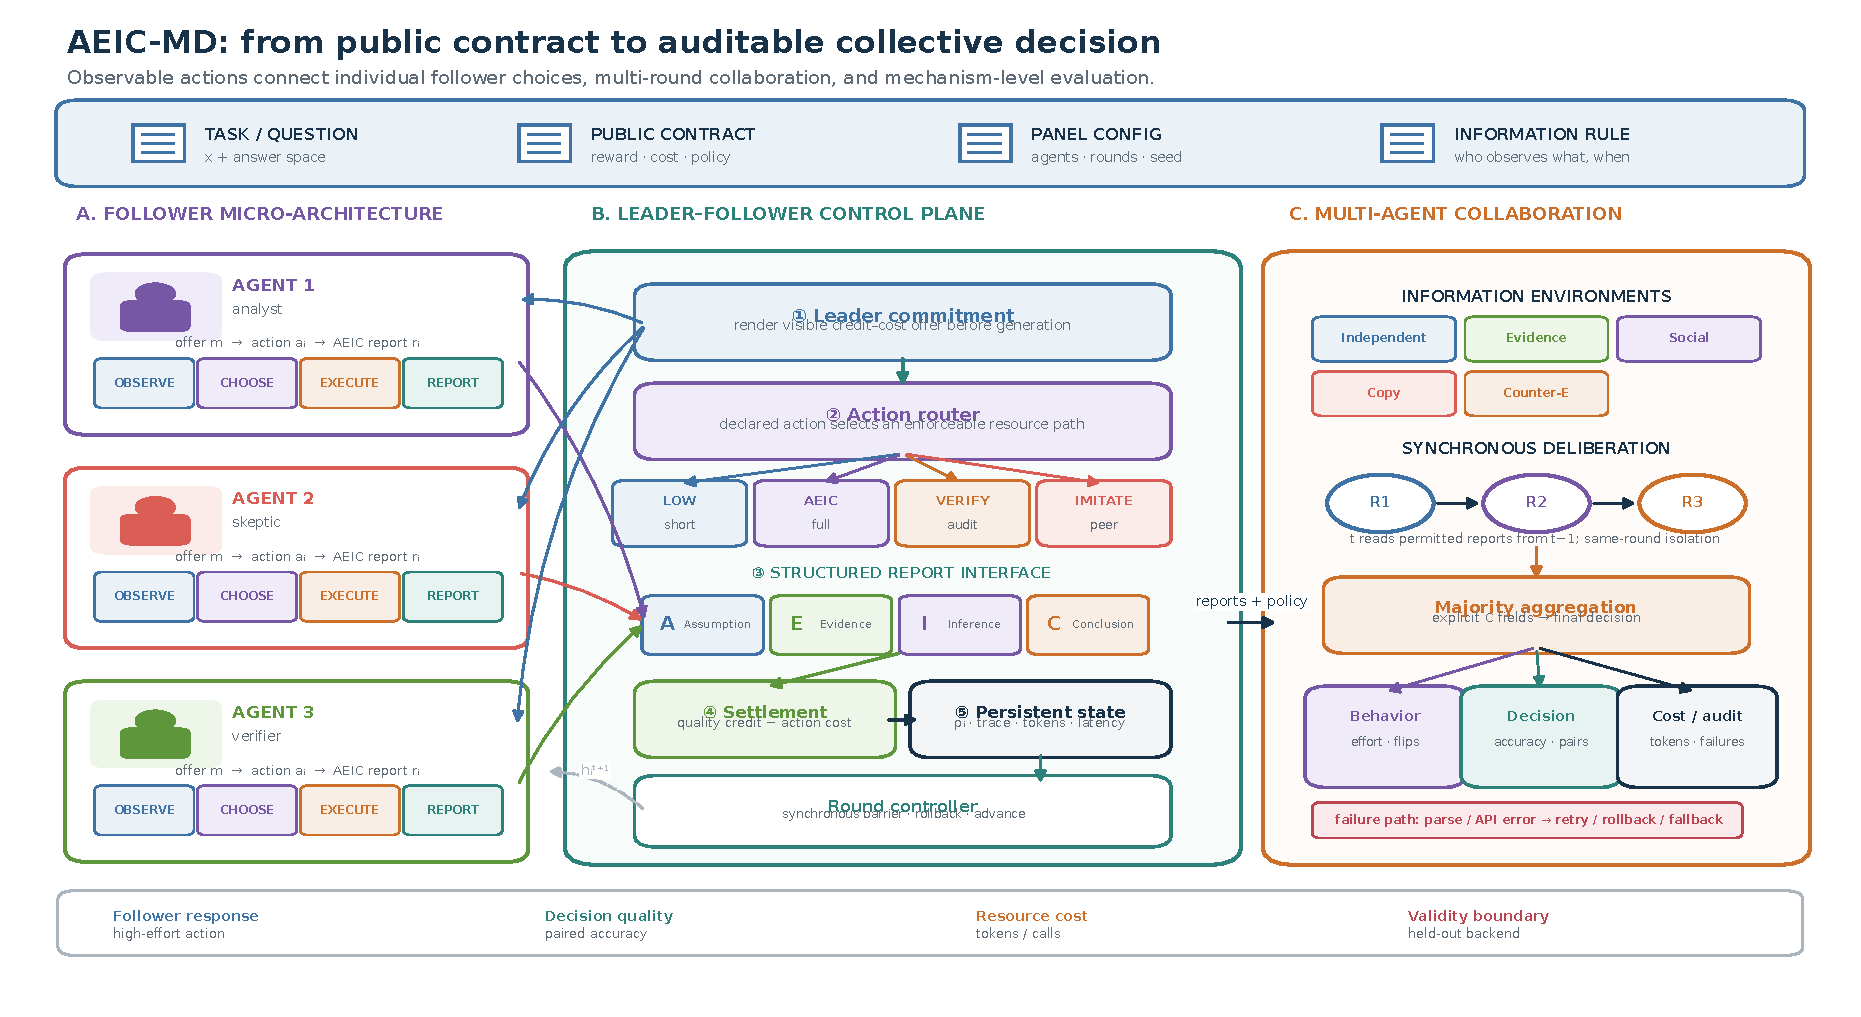
\includegraphics[width=\textwidth]{../figures/fig1_aeic_md_overview_rich.pdf}
\caption{AEIC-MD架构。合同先于资源行动选择，控制器在执行后结算并记录状态。}\label{fig:framework}\end{figure}

\section{实验协议与审计轨迹}\label{sec:protocol}
\paragraph{同步面板。}每道题由5个Agent进行3轮同步处理。第$t$轮只能观察策略允许的第$t-1$轮报告，同轮Agent彼此不可见。确认性实验使用独立信息条件；受控实验分别暴露新增证据、无证据多数立场、带复制压力的完整报告或立场相反证据。

图~\ref{fig:runtime}给出实现顺序：控制器先承诺，追随者声明行动，执行器运行对应路径，结算后才生成后续历史。失败进入可审计重试或回滚分支。
\begin{figure}[t]\centering
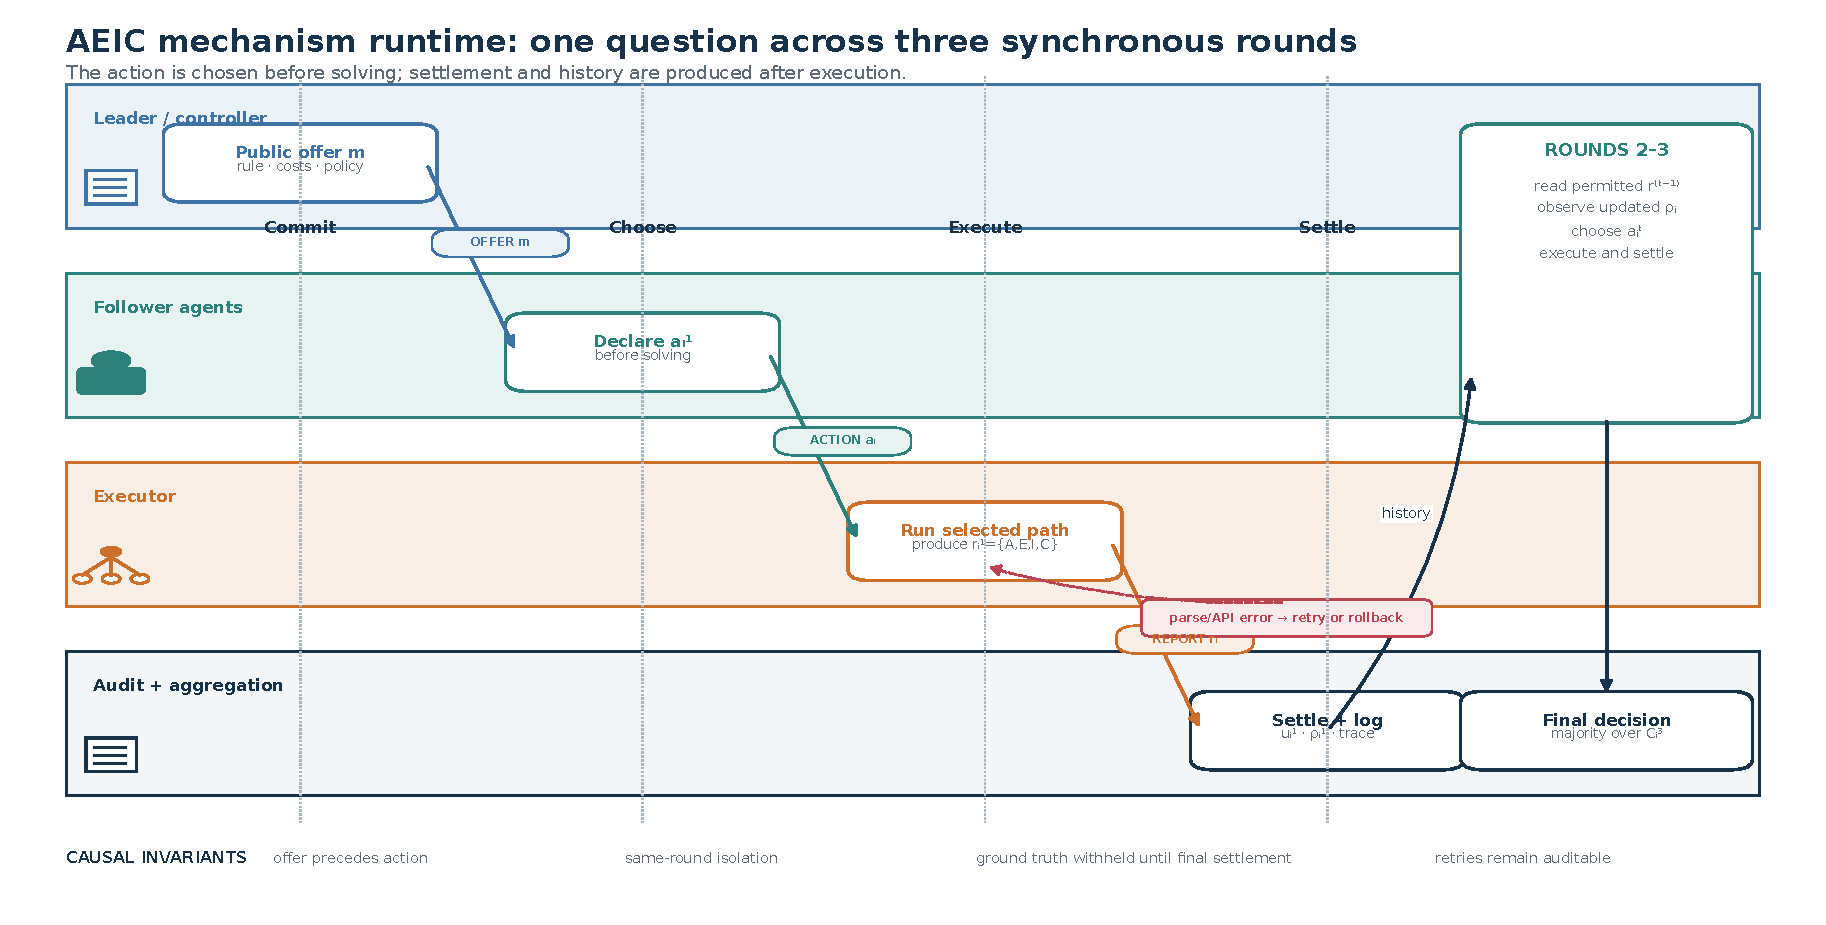
\includegraphics[width=\textwidth]{../figures/fig2_runtime_sequence.pdf}
\caption{单题运行时序。四条泳道区分承诺、选择、强制执行和结算。}\label{fig:runtime}\end{figure}

\paragraph{先选择后执行。}Agent先接收合同、信誉、允许信息和问题并返回单一行动；第二次调用执行行动，\textsc{Verify}增加审计与修订调用。仅解析失败时允许格式修复，且不得改变原结论或添加事实。

\paragraph{配对与聚合。}同一道题的机制共享问题级Seed。最终决策取第三轮$C$字段多数票。高资源行动预先定义为\textsc{AEIC}或\textsc{Verify}。二元结果使用精确McNemar检验，连续结果使用配对秩检验，并在注册比较族内Holm校正。

\paragraph{冻结溯源。}版本化Schema要求记录合同、行动、报告、可见同伴、奖励、成本、信誉、原始响应、Trace、延迟和Token。八组实验共5,850条问题级记录，均通过矩阵、路由和Schema校验，以SHA-256冻结并从标准JSONL独立复算。

\section{识别与结论边界}\label{sec:identification}
本文机制使用Stackelberg\emph{时序}而不声称闭式均衡：设计者承诺$m$，追随者再响应。AEIC是报告接口，而经验对象是黑盒策略诱导的行动分布$\pi(a\mid x,m,h)$。

\paragraph{追随者响应。}在配对任务上改变$m$并固定问题、Seed、面板、轮数和信息策略，可识别公开规则对已实现模型策略的意向处理效应。正的高资源行动差异证明规则响应，但不证明任意Agent效用最大化或激励相容。

\paragraph{仅结果控制。}Static AEIC与Outcome Only区分过程可观测性和一般奖励语言。它支持局部可检查接口是有效组成，但不隔离四个AEIC字段的独立贡献；信号消融只是描述性边界。

\paragraph{剂量响应。}式~\eqref{eq:followerutility}预测奖励提高时高资源行动弱增加、成本提高时弱降低。本文检验方向含义而不拟合结构效用模型；冻结高低点和开发中心点支持单调性，而非第二个确认性效应。

\paragraph{外部有效性。}Prompt介导的成本和信用具有后端语义，一个模型上的合同未必迁移到另一模型。因此本文将留出后端作为范围检验，不主张一般均衡、Leader全局最优、货币激励相容或拓扑无关有效性。

\paragraph{可证伪预测。}机制给出三个先验预测：其一，若Agent读取并响应过程合同，提高过程信用应使$\Pr(H(a)=1)$不下降；其二，提高同一行动的显式成本应使该概率不升高；其三，若效应来自可局部满足的生产规则而非一般奖励措辞，Outcome Only不应复制Static AEIC的行动响应。实验分别用奖励扫描、成本扫描和三条件确认性比较检验这些预测。预测失败将直接削弱机制解释，而不是被事后改写为提示效果。

\paragraph{可识别与不可识别部分。}确认性处理同时包含公开信用文本、行动选择Prompt和按行动分级的执行路径，因而能够识别这套可执行合同的总体效果，不能把准确率变化归因于单个字段。等计算量对照检验“只是多给Token”的替代解释；报告接口实验检验AEIC相对自由文本及一般结构化输出的增量；两者共同缩小解释范围，但仍不构成四字段的独立因果分解。

\section{实验}\label{sec:exp}
\subsection{实验设置}
我们从StrategyQA、MMLU-Hard和TruthfulQA各使用150道留出题。每个条件包含5个Agent和3轮同步审议，主后端为DeepSeek-V3~\cite{deepseek2024v3}。确认性实验包含$450\times3=1{,}350$条问题--条件记录和20,250个Agent-round。三种规则的问题、Seed、面板、轮数和聚合方式均配对，只有公开合同改变。最终决策取第三轮明确结论的多数票。

主要结果是高资源行动率（\textsc{AEIC}与\textsc{Verify}占比）和问题级准确率；同时报告每Agent-round Token、采集完整性和分域效应。配对二元结果采用精确McNemar检验，并在注册比较族内进行Holm校正。图~\ref{fig:evidence}概括识别逻辑和证据层级。
\begin{figure}[t]\centering
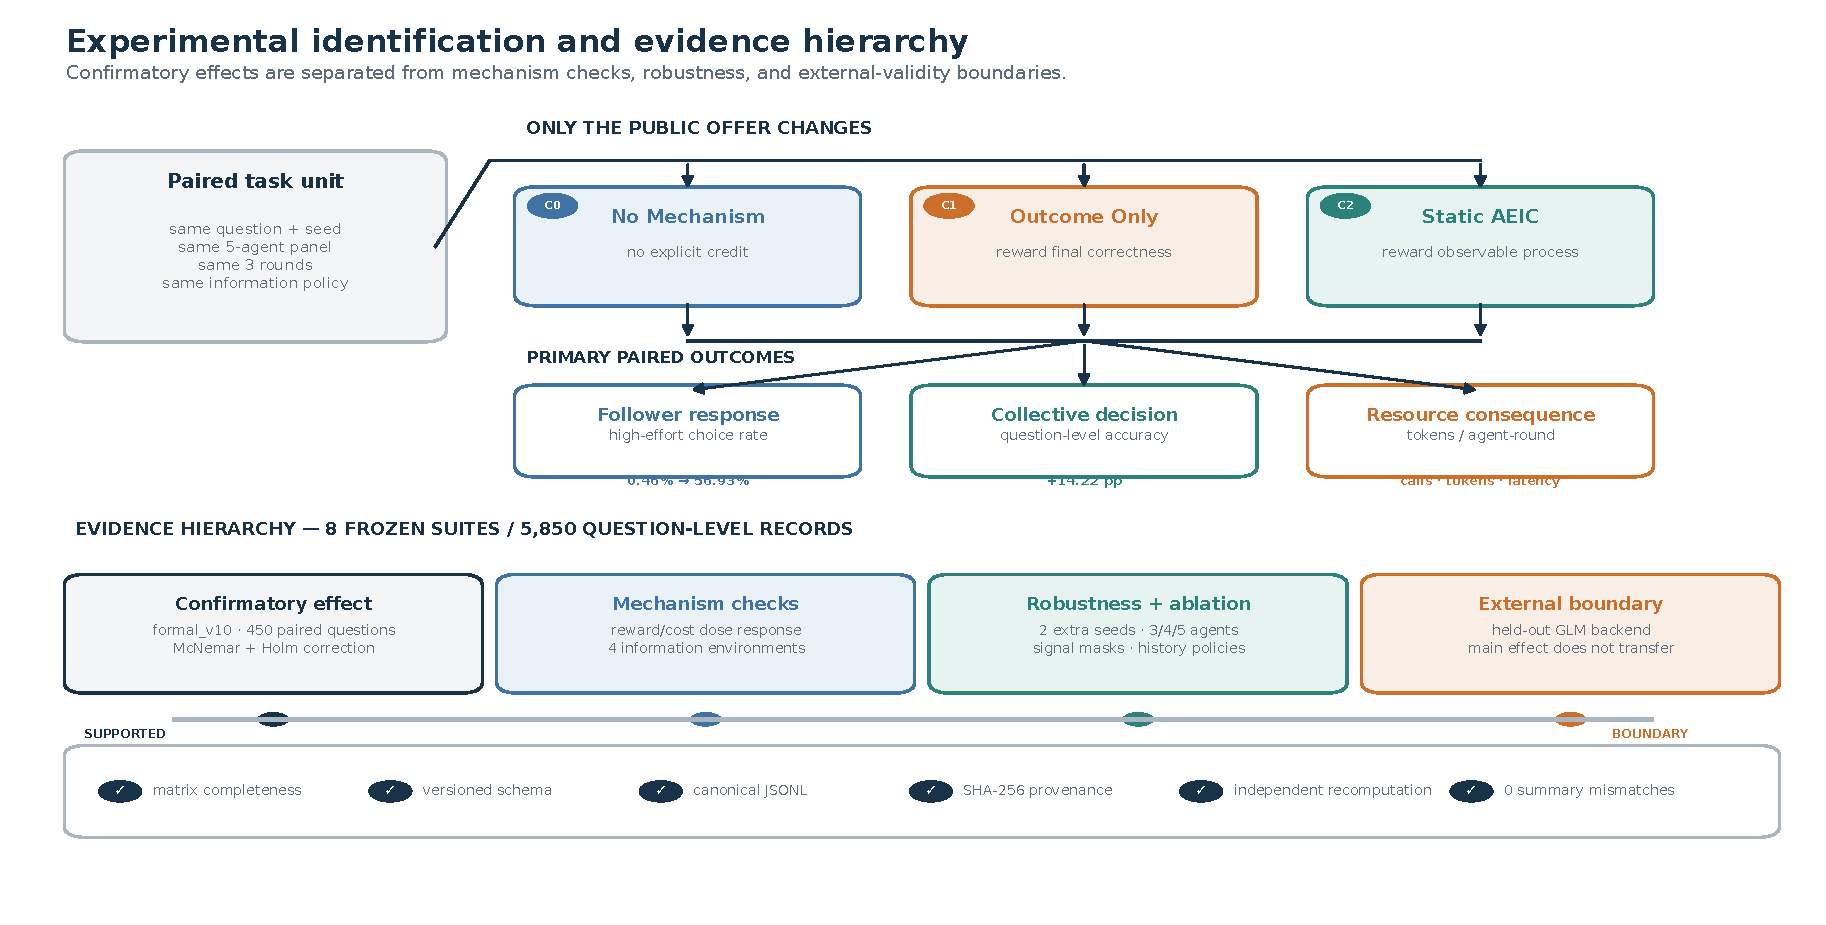
\includegraphics[width=\textwidth]{../figures/fig3_experimental_design.pdf}
\caption{实验识别与证据层级。配对条件隔离公开规则，八组冻结实验覆盖确认、机制检验、稳健性、消融与不迁移边界。}\label{fig:evidence}\end{figure}

\subsection{确认性追随者响应检验}
\begin{table}[t]
\caption{450道问题上的确认性配对检验。高资源行动在每种规则的6,750个Agent-round上测量。}\label{tab:main}
\centering\small
\begin{tabular}{@{}lccc@{}}\toprule
规则 & 高资源行动 & 准确率 & Token/Agent-round \\\midrule
No Mechanism & 0.46\% & 68.00\% & 663.3 \\
Outcome Only & 3.08\% & 67.33\% & 689.2 \\
Static AEIC & \textbf{56.93\%} & \textbf{82.22\%} & 808.8 \\\bottomrule
\end{tabular}\end{table}

Static AEIC同时改变追随者行为和集体决策（表~\ref{tab:main}；图~\ref{fig:formal}）。高资源行动率增加56.47个百分点；准确率增加14.22个百分点，相对No Mechanism有78道题由错变对、14道由对变错（Holm校正McNemar $p=1.23\times10^{-11}$）。每Agent-round额外145.5 Token与更完整工作的资源成本一致。

Outcome Only只将高资源行动率提高2.62个百分点，准确率变化$-0.67$个百分点（27道纠正、24道受损；$p=0.780$）。因此主效应不能概括为“告诉模型存在奖励”；区别在于规则是否提供追随者可通过生产过程满足的局部标准。
\begin{figure}[t]\centering
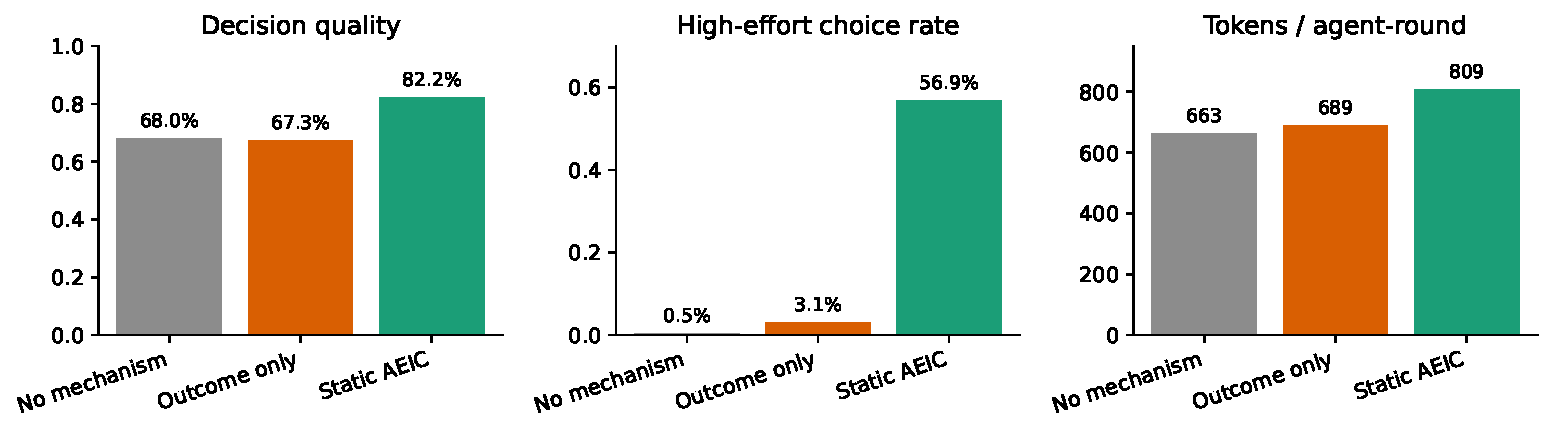
\includegraphics[width=\columnwidth]{../en/figures/fig1_formal_mechanism.pdf}
\caption{正式配对比较。基于AEIC接口的公开过程合同改变资源行动；合同、执行提示与分级资源路由的联合配置改善最终准确率，仅结果奖励没有改善准确率。}\label{fig:formal}\end{figure}

增益存在分域异质性：StrategyQA为$+4.0$、MMLU-Hard为$+20.0$、TruthfulQA为$+18.7$个百分点；对应高资源行动增益为43.5、73.7和52.2个百分点。因此总体效应不是任务无关常数。

从题目级流向看，Static AEIC相对No Mechanism产生78次错$\rightarrow$对和14次对$\rightarrow$错，净纠正64题。每题平均增加2,182 Token和0.80次调用，相当于每净纠正一题增加15,343 Token和5.64次调用。该结果正面呈现了质量收益的资源代价，而不是把准确率改善表述为免费收益。

\subsection{报告接口与机制成分分解}
为区分AEIC报告接口与合同执行效果，我们在90道配对问题上固定模型、调用次数和最大Token预算，比较自由文本、通用“分析--答案”结构和AEIC。三者准确率分别为72.22\%、82.22\%和85.56\%；AEIC相对自由文本提高13.33个百分点（Holm $p=0.00836$），但相对通用结构仅提高3.33个百分点（$p=0.453$）。因此AEIC的已证实作用是提供统一、可解析、可结算的语义接口；当前结果不支持其格式具有独立于一般结构化输出的准确率优势。

进一步在60道配对问题上固定DeepSeek后端，比较无合同固定资源、有合同固定资源、无合同匹配算力和完整机制。其高资源行动率分别为14.44\%、81.11\%、17.78\%和81.11\%，准确率分别为85.00\%、88.33\%、86.67\%和91.67\%。完整机制相对匹配算力将高资源行动提高63.33个百分点（$p=2.82\times10^{-33}$），实际Token差异不显著（$p=0.229$），说明行为响应不能由机械增加计算量解释。准确率差为$+5$个百分点，但仅有3次错$\rightarrow$对、0次对$\rightarrow$错（$p=0.25$），故只作为方向性成分证据。

\subsection{奖励--成本响应}
在每个任务域，奖励从0.05增至0.2和0.5时高资源行动单调不减；成本倍率从0.5增至1.0和1.5时单调不增（图~\ref{fig:boundary}）。冻结极值汇总中，高资源行动随奖励由49.42\%升至72.84\%，随成本由69.51\%降至53.78\%。中点来自同域开发观察，因此该实验是方向性机制检查而非第二个确认性效应。
\begin{figure}[t]\centering
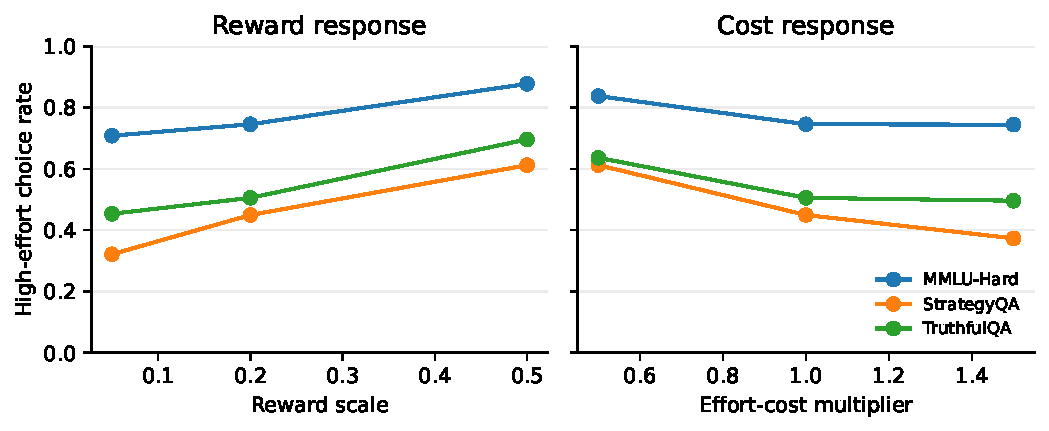
\includegraphics[width=\columnwidth]{../en/figures/fig2_incentive_response.pdf}
\caption{对公开合同的方向性响应：奖励提高时资源行动上升，行动成本提高时下降。}\label{fig:boundary}\end{figure}

\subsection{受控信息环境}
我们只改变第一轮后可见的同伴信息：新增证据、无证据多数立场、带复制压力的完整报告或立场相反证据。四类环境中，Static AEIC将汇总高资源行动率从0.86\%提高到49.41\%；各条件下为40.89\%--59.33\%，无机制时为0.44\%--1.47\%（图~\ref{fig:info}）。这说明接口在不同信息结构下仍有行为作用，但不证明每种信息干预都改善准确率或消除模仿。
\begin{figure}[t]\centering
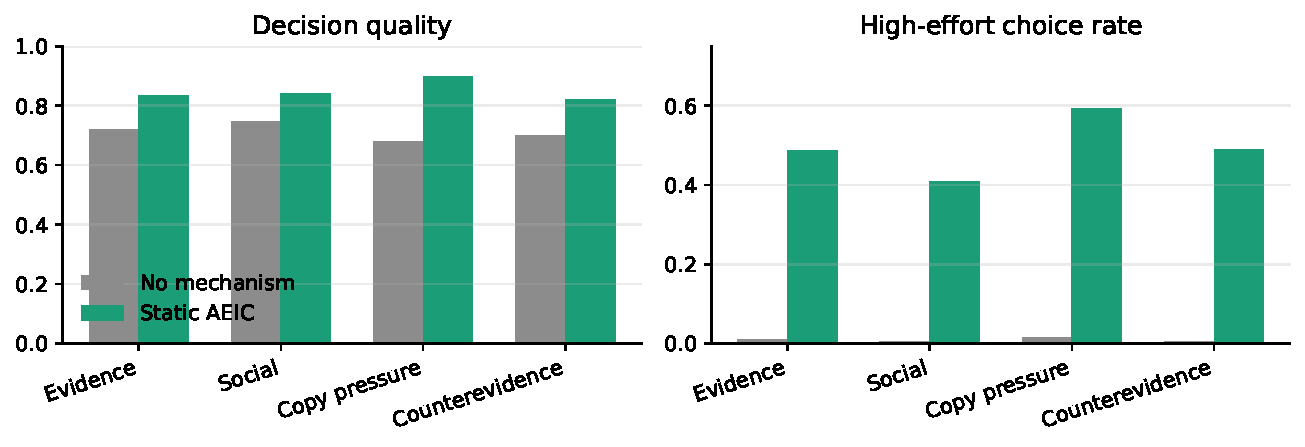
\includegraphics[width=\columnwidth]{../en/figures/fig3_information_conditions.pdf}
\caption{受控信息环境中的高资源行动。Static AEIC在四种设置中均改变行为。}\label{fig:info}\end{figure}

\subsection{稳健性、消融与外部有效性}
两个额外Seed复现主方向：Static AEIC准确率85.67\%，无机制71.00\%（$+14.67$个百分点；Holm校正$p=2.40\times10^{-9}$）。3、4、5 Agent条件下准确率为87.33\%--88.67\%。信号遮蔽和历史策略变体只限定当前实现，并不证明每个字段独立必要；移除字段会改变后端对整个合同的理解，因此属于干预消融而非模块化证明。
\begin{figure}[t]\centering
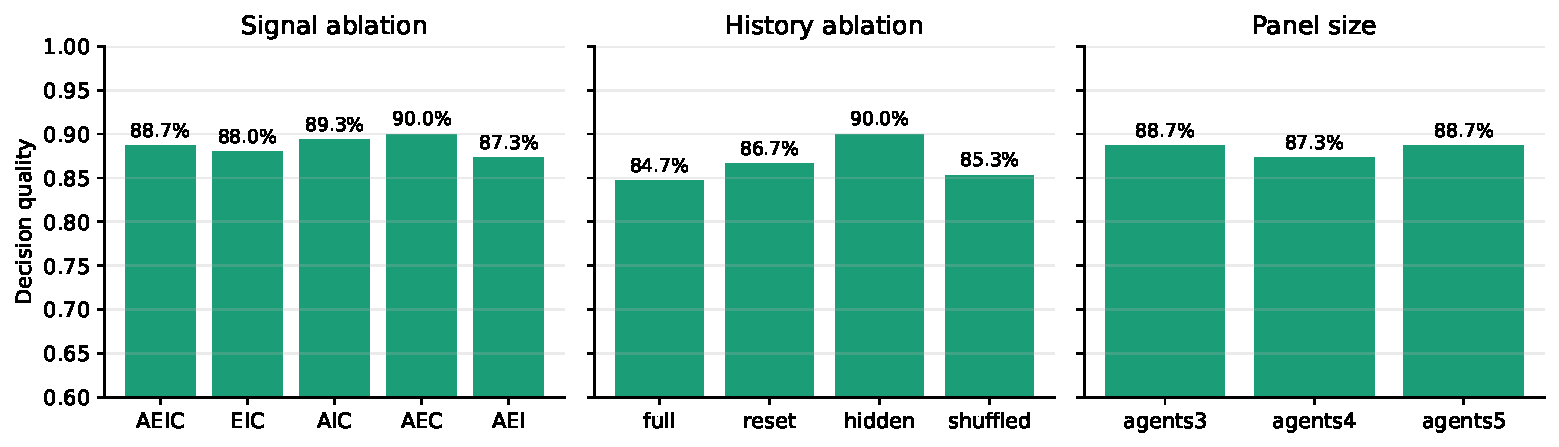
\includegraphics[width=\columnwidth]{../en/figures/fig4_ablations_robustness.pdf}
\caption{信号、历史、Seed与面板规模稳健性。组件变体是描述性边界。}\label{fig:robust}\end{figure}

留出GLM后端给出最强边界。Static AEIC仅将高资源行动率从0.58\%变为0.93\%（$p=0.134$），准确率为69.33\%，而无机制为70.67\%（Holm校正$p=0.791$）。相同文字和数值并不跨模型定义同一有效合同。当前公开过程合同仅在已测试主后端上得到实验支持，不是普适校准的激励语言。

\subsection{完整性与可复现性}
八组冻结实验的5,850条预期问题级记录全部存在；新增报告接口与机制拆解分别包含270和240条正式记录，总计6,360条。各冻结组通过Schema和路由验证，独立复算包与摘要无差异；机制拆解240条记录同样通过完整性检查。确认性数据中API终止失败为零、成本日志完整；少量解析失败经重试且保留在尝试日志。Manifest保存标准哈希，防止分析记录被静默替换。

\section{讨论}\label{sec:discussion}
\paragraph{机制而非格式本身。}AEIC的价值在于产生可缔约观测量，而非四个标签保证良好推理。Static AEIC在规则与观测量绑定时改变行为，Outcome Only说明一般奖励语言不足；但信号消融也不支持每个字段独立不可缺少的主张。

\paragraph{负迁移的重要性。}GLM结果表明，由Prompt介导的成本和信用通过后端特定策略解释，合同数值尚非通用货币。下一步应先在开发集估计各后端响应面，再在留出任务上测试固定合同；混合模型面板也应在解决校准后评估。

\paragraph{与拓扑和审议的关系。}生产激励决定是否产生信息性工作，通信拓扑决定谁能以何种成本观察这些工作。受控信息实验开始连接二者，却不把拓扑作为主因果变量。未来可在校准报告机制上优化信息流。

\paragraph{局限性。}主效应仅在一个主后端、三个二元答案QA域、一个Prompt行动菜单和多数聚合下建立。行动是LLM在指令下产生的行为，不代表类人偏好；信用是记账量而非货币；过程完整不等于事实验证。确认性实验检验固定静态规则，而非自适应Stackelberg最优性或一般均衡。更多调用和更长报告也带来真实计算成本。

\paragraph{更广泛含义。}该框架适用于中间工作可局部检查、执行器能够强制行动差异的场景，不应从结构完整但不可验证的报告制造虚假信心。因此记录合同、行动、执行路径和结算是贡献的一部分，而不只是工程日志。

\section{结论}\label{sec:conclusion}
本文把AEIC结构化报告作为Leader--Follower实验的可观测接口，并通过行动前公开合同与真实资源路径绑定构造语义共识机制。公开Static AEIC规则显著改变主后端的资源行动，联合执行配置下的集体准确率同时改善，仅结果奖励没有产生同样结果。受控信息实验支持AEIC信号的行为测量价值，但字段消融未证明单一字段独立必要，现有质量增益也不能归因于AEIC格式本身。剂量响应、稳健性实验和冻结溯源支持这一有边界的解释；留出后端失败进一步表明有效合同必须针对解释它的模型策略校准。后续识别顺序应是先验证报告接口，再分离合同与资源效应，最后进行有限合同选择。

因此，本文完成的是固定公开合同下Follower经验响应的识别，而不是一般Stackelberg均衡证明。其可复用贡献包括统一报告Schema、先选择后执行的资源约束、过程信号结算、跨轮信誉状态以及可复算Trace。未来工作将在冻结任务上估计奖励--成本响应面，定义包含质量、资源和失败风险的Leader效用，并只在有限合同空间中选择经验最优方案；任何新合同均需在独立任务和新模型后端上重新校准与验证。


\bibliographystyle{splncs04}
\bibliography{references}

\end{document}
